\section{Exercise 1 - Data structures}
The first problems we need to solve is which data structures should be used for our abstract syntax tree, which will serve as the first step of our intermediate representation.

\subsection{Abstract syntax tree data structure}
We have decided that we could use an unbalanced tree for storage of our abstract syntax tree in our target programming language. Constraining the tree construction will give us the necessary check for syntax errors.
A simple tree-traversal will give us the appropriate unique label numbers.

\subsection{Data structure}
In our implementation language the statements from the \texttt{WHILE} language will be mapped into objects. 
\\\\
We will have the following objects.
\begin{itemize}
	\item \textbf{Declaration} - Figure~\ref{fig:declaration} shows the structures of declarations.
	\item \textbf{Statement} - Figure~\ref{fig:statement} shows the structures of statements.
	\item \textbf{Variable} - Figure~\ref{fig:variable} shows the structures of variables.
	\item \textbf{Condition} - Figure~\ref{fig:condition} shows the structures of conditions.
	\item \textbf{Expression} - Figure~\ref{fig:expression} shows the structures of expressions.
\end{itemize}

\begin{figure}[h]
	\centering
	\includegraphics[scale=.3]{../fig/Declaration}
	\caption{Declarion}
	\label{fig:declaration}
\end{figure}

\begin{figure}[h]
	\centering
	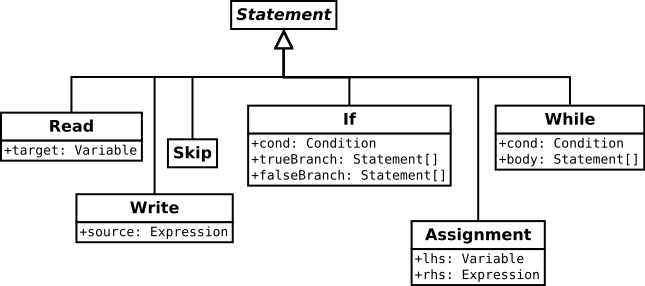
\includegraphics[scale=.3]{../fig/Statement}
	\caption{Statement}
	\label{fig:statement}
\end{figure}

\begin{figure}[h]
	\centering
	\includegraphics[scale=.3]{../fig/Variable}
	\caption{Variable}
	\label{fig:variable}
\end{figure}

\begin{figure}[h]
	\centering
	\includegraphics[scale=.3]{../fig/Condition}
	\caption{Condition}
	\label{fig:condition}
\end{figure}

\begin{figure}[h]
	\centering
	\includegraphics[scale=.3]{../fig/Expression}
	\caption{Expression}
	\label{fig:expression}
\end{figure}

\subsection{Flow graph data structure}
For the flow graph, we have chosen a network graph data structure. This gives an intuitive way of linking statements to potential paths.
\\
\\
It is convenient to transform the abstract syntax tree into a flow graph when performing a program analysis. For that reason a data structure for the flow graph as well as mapping from a abstract syntax tree to a flow graph is needed 
\\
\\
Figure~\ref{fig:flowgraph} shows the classes used to represent a flow graph. The idea is that there exists two kinds of nodes that both inherits from the abstract \texttt{Node} class. Each \texttt{Node} has a \texttt{label} and a \texttt{prev}, which is the previous node in the graph. The first node in the program will not have a previous node. A \texttt{Statement Node} is a node that contains a \texttt{CodeBlock} and it is used for everything that does not use branching. It has a pointer to the next node in the flow graph. A \texttt{Branching Node} is used for if statements and while loops where branching is needed. It contains a \texttt{condition} and a pointer to two possible next nodes.

\begin{figure}[h]
	\centering
	\includegraphics[scale=1.0]{../img/flow_graph}
	\caption{Data structures used to represent a flow graph}
	\label{fig:flowgraph}
\end{figure}

\subsubsection{Creating flow graphs}
The way a flow graph representation will be created is by first going through all declarations in the abstract syntax tree. This will for sure not include branching so they should end up in \texttt{Statement Node}s. One for each declaration. The next thing to do is to go through each statement and check whenever it is a branching statement or not and create the correct nodes. When a statement is met that contains more statements (for instance a while statement), these statements needs to be added to the graph before the iteration of statements can continue.


\subsection{Program graph data structure}
For some types of analysis it is more convenient to use a program graph compared to a flow graph. In that case a way of transforming a abstract syntax tree into a program graph is needed. Figure~\ref{fig:programgraph} shows a data structure for a program graph. It is a bit more complicated than flow graphs since we need to introduce both nodes and edges. A node has a \texttt{label}. If it is a \texttt{Branch Node} then it contains two \texttt{Branch Edge}s. A \texttt{Branch Edge} is an edge that contains a \texttt{condition}. If it is a \texttt{Statement Node} is contains a \texttt{Statement Edge}. A \texttt{Statement Edge} is an edge that contains a \texttt{codeBlock}.

\begin{figure}[h]
	\centering
	\includegraphics[scale=1.0]{../img/program_graph}
	\caption{Data structures used to represent a program graph}
	\label{fig:programgraph}
\end{figure}

\subsubsection{Creating program graphs}
A program graph can be created much in the same way as a flow graph by going through all the declarations first and then the statements. Basically the only difference is that the labels are stored in nodes and code blocks and conditions are stored in edges.